\documentclass[final]{article}

% if you need to pass options to natbib, use, e.g.:
% \PassOptionsToPackage{numbers, compress}{natbib}
% before loading nips_2017
%
% to avoid loading the natbib package, add option nonatbib:
% \usepackage[nonatbib]{nips_2017}

\usepackage{nips_2017}
\usepackage{graphicx,url}
\usepackage{amsmath}
\usepackage{amssymb}
\usepackage{balance}
\usepackage{gensymb}
\usepackage{multirow}
\usepackage{hhline}
\usepackage{array}
\usepackage[font=small,labelfont=bf]{caption}
\usepackage{dblfloatfix}
\usepackage{gensymb}
% to compile a camera-ready version, add the [final] option, e.g.:
% \usepackage[final]{nips_2017}

\usepackage[utf8]{inputenc} % allow utf-8 input
\usepackage[T1]{fontenc}    % use 8-bit T1 fonts
\usepackage{hyperref}       % hyperlinks
\hypersetup{
    colorlinks=true,
    linkcolor=blue,
    filecolor=magenta,      
    urlcolor=blue,
}
\usepackage{url}            % simple URL typesetting
\usepackage{booktabs}       % professional-quality tables
\usepackage{amsfonts}       % blackboard math symbols
\usepackage{nicefrac}       % compact symbols for 1/2, etc.
\usepackage{microtype}      % microtypography

\title{Assignment 2 - Localization with Particle Filters}

% The \author macro works with any number of authors. There are two
% commands used to separate the names and addresses of multiple
% authors: \And and \AND.
%
% Using \And between authors leaves it to LaTeX to determine where to
% break the lines. Using \AND forces a line break at that point. So,
% if LaTeX puts 3 of 4 authors names on the first line, and the last
% on the second line, try using \AND instead of \And before the third
% author name.

\author{
  Patrick Lancaster\\
  Paul G. Allen School of Computer Science and Engineering\\  
  University of Washington\\
  Seattle WA, 98195 \\
  \texttt{planc509@cs.washington.edu} \\
  \And
  Arunkumar Byravan\\
  Paul G. Allen School of Computer Science and Engineering\\
  University of Washington\\
  Seattle WA, 98195 \\
  \texttt{barun@cs.washington.edu} \\ 
  \And
  Kendal Lowrey\\
  Paul G. Allen School of Computer Science and Engineering\\
  University of Washington\\
  Seattle WA, 98195 \\
  \texttt{klowrey@cs.washington.edu} \\    
  %% examples of more authors
  %% \And
  %% Coauthor \\
  %% Affiliation \\
  %% Address \\
  %% \texttt{email} \\
  %% \AND
  %% Coauthor \\
  %% Affiliation \\
  %% Address \\
  %% \texttt{email} \\
  %% \And
  %% Coauthor \\
  %% Affiliation \\
  %% Address \\
  %% \texttt{email} \\
  %% \And
  %% Coauthor \\
  %% Affiliation \\
  %% Address \\
  %% \texttt{email} \\
}

\begin{document}
%\nipsfinal

\maketitle

\section{Introduction}

In this assignment you will implement a particle filter to localize your car within a known map. This will provide a global pose ($\mathbf{x_t} = <x_t, y_t, \theta_t>$) for your car where ($x_t$, $y_t$) is the 2D position of the car within the map and $\theta_t$ is the heading direction w.r.t the map's frame of reference. You will be implementing different parts of the particle filter, namely the motion model, sensor model, and the overall filtering framework. You will also be tuning various parameters that govern the particle filter to gain intuition on the filter's behaviour. The provided \href{https://gitlab.cs.washington.edu/uw_racecar/course_materials/lab2}{skeleton code} has some code to get you started, as well as data and code for testing different aspects of your particle filter. 

This assignment can be done as a group. Only one member of the group needs to submit it to the Canvas dropbox. All group members' names should be on the document containing answers to the assignments' questions.

\section{Getting Started}

Here is some \textbf{very important} prerequisite information for this assignment:

\begin{itemize}

\item Many of the comments in the skeleton code specify that a computation should be done \textit{in-place}, particularaly when updating \texttt{self.particles} and/or \texttt{self.weights}. For example, updating the \texttt{self.weights} \textit{in-place} means that the result of the update should be stored in the \texttt{self.weights} array, rather than returning a new array that contains the result of the update. Note that, at least in this context, doing an in-place update does not mean that you cannot use intermediate arrays and/or data structures to perform the calculation. It only specifies that the values of an array (such as \texttt{self.particles} or \texttt{self.weights}) should be updated with the result of the computation, rather than returning a whole new array.

\item Emphasizing the point above, when updating the values of \texttt{self.particles} and/or \texttt{self.weights}, make sure that you are updating the \textit{values} of the array, rather than changing the array that \texttt{self.particles} and/or \texttt{self.weights} refers to. Different modules each contain their own references to \texttt{self.particles}, but they all refer to the same array (the same can be said for \texttt{self.weights}). Therefore changing the array that \texttt{self.particles} and/or \texttt{self.weights} references in one module will cause the other modules to no longer see the updates made by that module (and vice-versa). For example, doing something of the form \texttt{self.weights = a} would be very bad; instead one could use \texttt{self.weights[:] = a[:]} to update the \texttt{self.weights} array.

\item The particle filter algorithm that we wrote in class contains a number of for-loops. However, for most of these for-loops, the iterations are independent of each other. Therefore we can turn many of these for-loops into vector computations. For example, instead of sampling particles one at a time from the motion model, you can receive a whole vector of sampled particles. You should do vectorized computations whenever possible in order to write efficient code - failing to do so could cause your particle filter to not run sufficiently fast.

\item Note that, in another deviation from the particle filter algorithm we wrote in class, the particles and weights are updated asynchronously. Specfically, the motion model is applied whenever messages about the speed of the motor and steering angle are received. The sensor model is applied whenever a laser scan is received, which also triggers the weighted re-sampling of particles shortly after. This asynchronous structure allows us to utilize all of the messages that are received, rather than operating at the rate of the slowest topic.

\item We have provided code to help visualize the output of your motion and sensor models. Before trying to run the whole particle filter, we strongly suggest that you test your motion model and sensor model individually by using these visualizations to validate that their output makes sense. More details about how to run these visualizations are given in relevant sections of the assignment.

\end{itemize}

\section{ Motion Model}
As discussed in class, a motion model specifies the probability distribution $p(\mathbf{x}_t | \mathbf{x}_{t-1}, u_t)$, i.e. the probability of reaching a pose $\mathbf{x}_t$ given that we apply a control $u_t$ from pose $\mathbf{x}_{t-1}$. Unlike a traditional Bayes filter which requires us to explicitly represent the posterior over possible future poses (i.e. explicitly compute $p(\mathbf{x}_t | \mathbf{x}_{t-1}, u_t)$),  we only need to be able to draw samples from this distribution for the particle filter:
\begin{equation}
\mathbf{x}^\prime_t \sim p(\mathbf{x}_t | \mathbf{x}_{t-1}, u_t) 
\end{equation}
where $\mathbf{x}^\prime_t$ is a possible next pose ($x_t,y_t,\theta_t$) sampled from the motion model.

\subsection{Kinematic Model}
We can explicitly derive a motion model based on the kinematic structure of the car. As we discussed in class, our controls for the racecar are the speed of the car $v$ and its steering angle $\delta$, i.e. $u_t = <v_t, \delta_t>$. The kinematic car model explicitly models the effect of this action $u_t$ on the previously estimated robot pose $\mathbf{x}_{t-1}$ to get the future pose $\mathbf{x}_t$. Further details on the derivation of this model are provided below (and in the class notes):

%As derived in class, the kinematic model depends on the width of the front wheels and the length of the car.

\begin{align*}
x_t =& x_{t-1} + \frac{L}{\sin{2\beta}}(\sin{\theta_t} - \sin{\theta_{t-1}}) \\
y_t =& y_{t-1} + \frac{L}{\sin{2\beta}}(-\cos{\theta_t} + \cos{\theta_{t-1}}) \\
\theta_t =& \theta_{t-1} + \frac{v}{L}\sin{(2\beta)} \Delta t \\
\beta =& \arctan( \frac{1}{2}\tan{\delta}) \\
\end{align*}

\begin{figure}[h]
\noindent\begin{minipage}{.75\textwidth}
   % \centering
%    \rule{4cm}{3cm}
   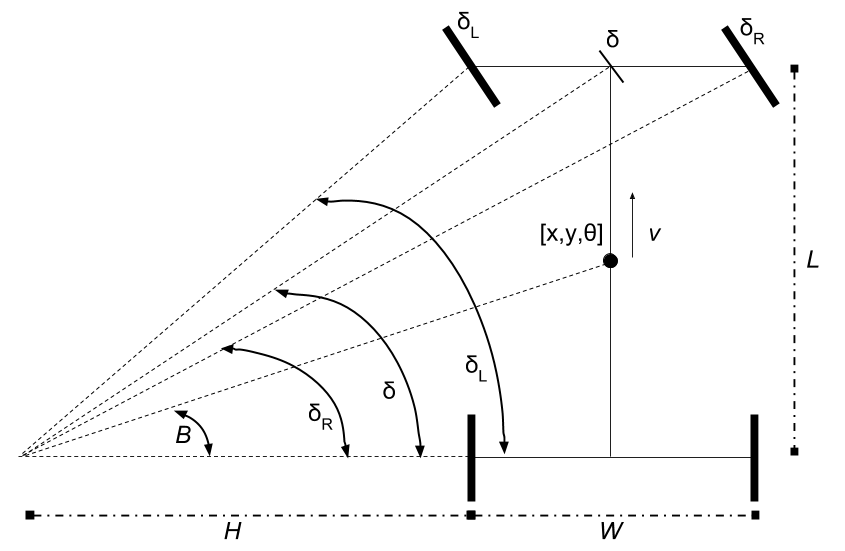
\includegraphics[width=1.0\textwidth]{figs/kinematic_car_model.png}
%    \caption{Kinematic Car Model}
\end{minipage}
\begin{minipage}{.15\textwidth}
\begin{align*}
   \tan{\delta_r} =& \frac{L}{W+H}\\
   \tan{\delta_l} =& \frac{L}{H}\\
   \tan{\delta} =& \frac{L}{H+W/2}\\
   \tan{\beta} =& \frac{L/2}{H+W/2}\\
\end{align*}
\end{minipage}
\caption{Simplified Kinematic Model of the robot car. State consists of position and heading angle ($x$, $y$, $\theta$). Controls consist of velocity and steering angle ($v$, $\delta$).}
\end{figure}

\subsection{Noise}

The kinematic car model makes deterministic predictions, i.e. given an initial pose $\mathbf{x}_{t-1}$ and control $u_t$ there is a single predicted future pose $\mathbf{x}_t$. This would be acceptable if our model is perfect, but as you have seen we have made many simplistic assumptions to derive this model. In general, it is very hard to model any physical process perfectly. In practice, we would like our model to be robust to  potential errors in modeling. We do this by allowing our model to be probabilistic - given any pose $\mathbf{x}_{t-1}$ and control $u_t$, our model can predict a distribution over future states $\mathbf{x}_t$, some being more likely than others. We achieve this by sampling noisy controls from the nominal controls $\bar{v_t}$ and $\bar{\delta_t}$, propogating those controls through the kinematic car equations to get prediction $\bar{x_t} = f[x_{t-1},u_t]$, and finally adding model noise to the output. Mathematically: 

\begin{align*}
u_t =& <v_t, \delta_t>, v_t \thicksim N(\bar{v_t},\sigma_v), \delta_t \thicksim N(\bar{\delta_t}, \sigma_{\delta}) \\
\bar{x_t} =& f[x_{t-1},u_t] \\
x_t \thicksim & N(\bar{x_t}, \sigma_{x_t})
\end{align*}

It is up to you to pick reasonable noise parameters that determine the widths of the various gaussians that must be sampled from. You should implement the motion model in the provided \textbf{MotionModel.py} script. \textbf{Make sure to vectorize computation whenever possible.}

\subsection{Motion Model Visualization}
The code for visualization of the motion model is given in the main function of \textbf{MotionModel.py}. First make sure that \textbf{teleop.launch is NOT running}. Then launch \textbf{MotionModel.launch}. A gui window will then pop up, where a red dot will specify the initial positions of the particles (they are all at (0,0)), and blue dots specify the position of the particles after one time step. The speed, steering angle, and time step length are all controlled by variables specified right above the main function. Vary these values and verify that the particles propagate forward as expected. Fig. \ref{fig:motion_model} is an example of what you might expect to see when the robot is told to turn left at a speed of 1.0 m/s for one second (given our implementation's noise parameters).

\begin{figure*}[h]
\centering
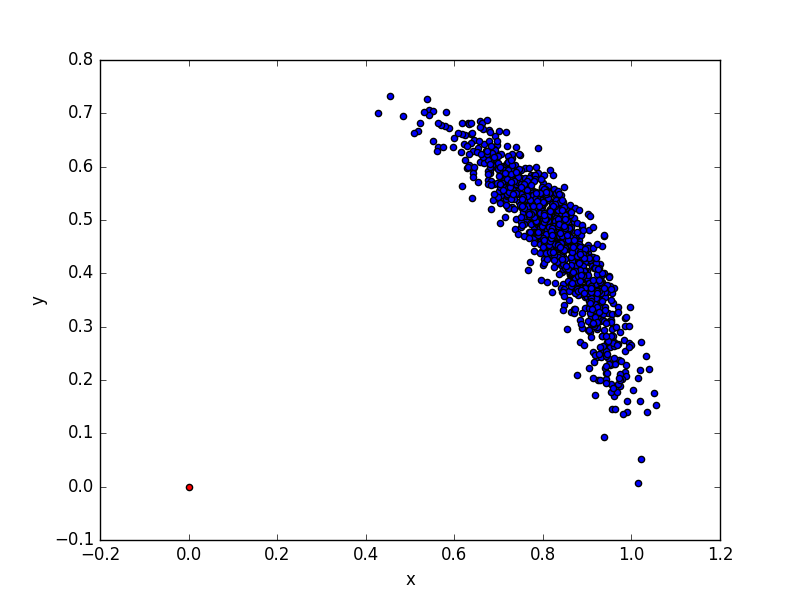
\includegraphics[width=0.45\linewidth]{figs/motion_model.png}
\caption{Propagation of particles when moving forward and to the left.}
\label{fig:motion_model}
\end{figure*}

\section{Sensor Model}

The sensor model captures the probability $p(\mathbf{z}_t | \mathbf{x}_t)$ that a certain observation $\mathbf{z}_t$ can be obtained from a given robot pose $\mathbf{x}_t$ (assuming that the map of the environment is known). In this assignment, $\mathbf{z}_t$ is the LIDAR data from the laser sensor mounted on the robot. Your task in this section is to implement and analyze the LIDAR sensor model discussed in class.

\subsection{Model}
The LIDAR sensor shoots out rays into the environment at fixed angular intervals and returns the measured distance along these rays (or NAN and/or 0.0 for an unsuccesful measurement). Therefore, a single LIDAR scan $\mathbf{z}$ is a vector of distances along these different rays $\mathbf{z} = \left[z^1, z^2, ...., z^N\right]$. Given the map of the environment ($m$), these rays are conditionally independent of each other, so we can rewrite the sensor model likelihood as follows:
\begin{align}
p(\mathbf{z}_t | \mathbf{x}_t, m) = p(z_t^1, z_t^2, ...., z_t^N | \mathbf{x}_t, m) = p(z_t^1 | \mathbf{x}_t, m) * p(z_t^2 | \mathbf{x}_t, m) * ... * p(z_t^N | \mathbf{x}_t ,m )
\end{align}
where the map $m$ is fixed (we will not use $m$ explicitly in any further equations, it is assumed to be provided). As we can see, to evaluate the likelihood it is sufficient if we have a model for measuring the probability $p(z_t^k | \mathbf{x}_t)$ of a single range measurement given a pose . 

We will compute this in the following manner: First, we will generate a simulated observation $\hat{\mathbf{z}}_t$ given that the robot is at a certain pose $\mathbf{x}_t$ in the map. We do this by casting rays into the map from the robot's pose and measuring the distance to any obstacle/wall the ray encounters. This is very much akin to how laser light is emitted from the LIDAR itself. We then quantify how close each ray in this simulated observation $\hat{\mathbf{z}}^k_t$ is to the real observed data $\mathbf{z}^k_t$, which provides an estimate of $p(z_t^k | \mathbf{x}_t)$. 

Overall, this requires two things: 
\begin{enumerate}
\item A way to compute the simulated observation given a pose
\item A model that measures closeness between the simulated and real data
\end{enumerate}

For the purpose of this assignment, we will use a raycasting library called rangelibc (implemented in C++/CUDA) to compute the simulated observation. The second part is what you will be implementing - a model that measures how likely you are to see a real observation $\mathbf{z}^k_t$ given that you are expected to see a simulated observation $\hat{\mathbf{z}}^k_t$. The LIDAR sensor model we use is a combination of the following four curves, with certain mixing parameters and hyper-parmeters that weight each of the four components against the other that will be chosen by you. More details on this model can be found in Section 6.3.1 of \textit{Probabilistic Robotics} as well as in the lecture notes.

\begin{figure}[h]
\centering
%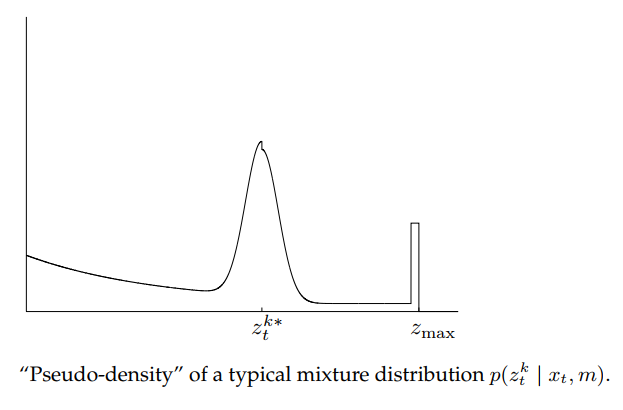
\includegraphics[width=10cm]{s_model.PNG}
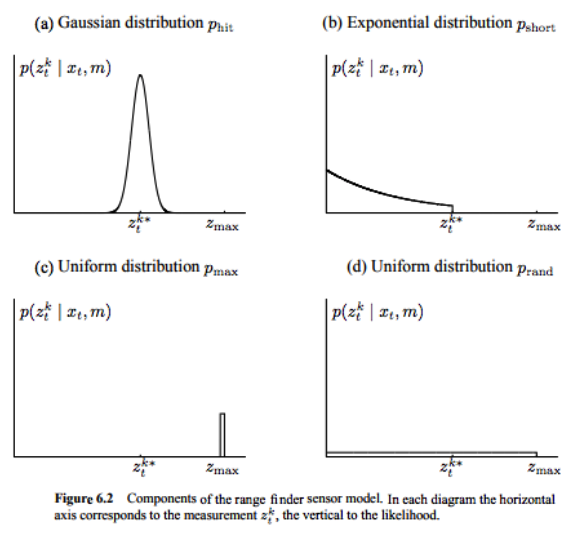
\includegraphics[width=11cm]{figs/s_noise.png}
\end{figure}

Given that the LIDAR range values are discrete (continuous values are converted to discrete pixel distances on the 2D map), we do not have to generate the model on-line and can instead pre-calculate them. This will be represented as a table of values, where each row is the actual measured value and the column is the expected value for a given LIDAR range. Pre-computing this table allows for faster processing during runtime. During run-time, we use the aforementioned ray casting library to generate simulated range measurements. This is then used in your calculated look-up table, and compared to the LIDAR output.

For this part of the assignment, you will implement the sensor model in the file \textbf{SensorModel.py}. In particular, the function \texttt{precompute\_sensor\_model()} should return a \texttt{numpy} array containing a tabular representation of the sensor model. The code provided will use your array as a look-up table to quickly compare new sensor values to expected sensor values, returning the final sensor model likelihood: $p(\mathbf{z}_t | \mathbf{x}_t)$. In addition, due to the density of the laser scans, you will down-sample the received scan in order to reduce the amount of necessary computation. More details can be found in \textbf{SensorModel.py}. \textbf{Make sure to vectorize computation whenever possible.}

\subsection{Sensor Model Visualization}
The code for visualization of the sensor model is given in the main function of \textbf{SensorModel.py}. Open \textit{racecar\_base\_public/racecar/launch/includes/common/map\_server.launch} and change the \textit{map} argument to reference the \textit{sieg\_floor3} map. Then make sure that  \textbf{teleop.launch is NOT running}. Finally, launch \textbf{SensorModel.launch}. This will play back a bag file that contains a laser scan taken from somewhere in the map. The code will then exhaustively  compute $p(\mathbf{z}_t | \mathbf{x}_t)$ for every pose in the map. It will return a heatmap illustrating which locations are most likely. We provide three bag files to try your sensor model out on. The path of the bag file is specified in \textbf{SensorModel.launch}. The expected outputted heatmaps for each bag (as well the bags themselves) can be found in \textit{lab2/bags/laser\_scans}. Note that your results will differ depending on the sensor model parameters that you choose. If the code reports a memory error or the node dies after printing out 
\textit{'Done, preparing to plot'}, try increasing the amount of RAM allocated to your VM.
\section{Particle Filter}

The bayes filter consists of a motion model that predicts the movement of the robot, and compares the expected sensor values after this movement to the sensor values collected from the real robot. In the particle filter, your belief over the robot pose $Bel(\mathbf{x}_t)$ is represented as a list of $M$ particles (these are nothing but samples from the belief distribution). Each particle $i$ has a pose $\mathbf{x}^i_t$ which represents a hypothetical robot at that particular pose; using many particles allows for us to more accurately represent the belief distribution. 

\subsection{Implementation}

In this part of the assignment, you will be implementing a particle filter to track our belief over the robot's pose over time with a fixed number of particles. The code from the prior sections will be used in the file \textbf{ParticleFilter.py}. 

From a high level, this is how the particle filter works. Initially, we have a prior belief over where the robot is: $Bel(\mathbf{x}_0)$. You are provided with a clicking interface that enables you to specify the initial pose of the robot - this will specify $Bel(\mathbf{x}_0)$. We will represent this belief using a fixed number of $M$ particles - initially all these particles will be gaussian distributed around the clicked pose. In order to specify a pose, look for a button labeled '2D Pose Estimate' along the top bar of the RVIZ interface. After clicking this button, you  can specify a position and orientation by clicking and dragging on the map. Next, each particle will be propagated forward in time using the motion model. Using ray-casting, we will generate a simulated LIDAR observation for each particle which we will compare to the real LIDAR data from the laser sensor. This now assigns a ``weight'' for each particle - particles with higher weights are more likely given the motion and sensor model updates. Finally, we will re-sample from this distribution to update our belief over the robot's pose $Bel(x_t)$ - this resampling step gets rid of particles with low belief and concentrates our distribution over particles with higher belief. We repeat these steps recursively. You will implement functions in \textbf{ParticleFilter.py} to initialize the belief, as well as compute the expected pose of the robot. See the skeleton code for more details.

In prior sections, you implemented algorithms for sampling from a motion model with noise and evaluating a sensor model. The key step remaining is to implement the re-sampling step (discussed in the next section) and to connect all the parts together in a tight loop that should run in real-time. 

%The particle filter's re-sampling step is then performed, and when needed, a $x$, $y$, $\theta$ can be calculated that represents the car's location.

\subsection{Re-sampling}
You will implement two re-sampling procedures for your particle filter in \textbf{ReSample.py}. First is the naiive re-sampler: If we have $M$ particles, we create $M$ bins, each of which has a width equal to the corresponding weight. We then draw $M$ random numbers between 0.0 and 1.0, and for each of those numbers, return the particle that corresponds to the bin that the random number falls into. (Hint: \texttt{np.random.choice} is a good place to start.)

The second re-sampler is a low-variance re-sampler, which only draws a single random number. This is detailed in table 4.4 from \textit{Probabilistic Robotics} and implemented as follows:

\begin{figure}[h]
\centering
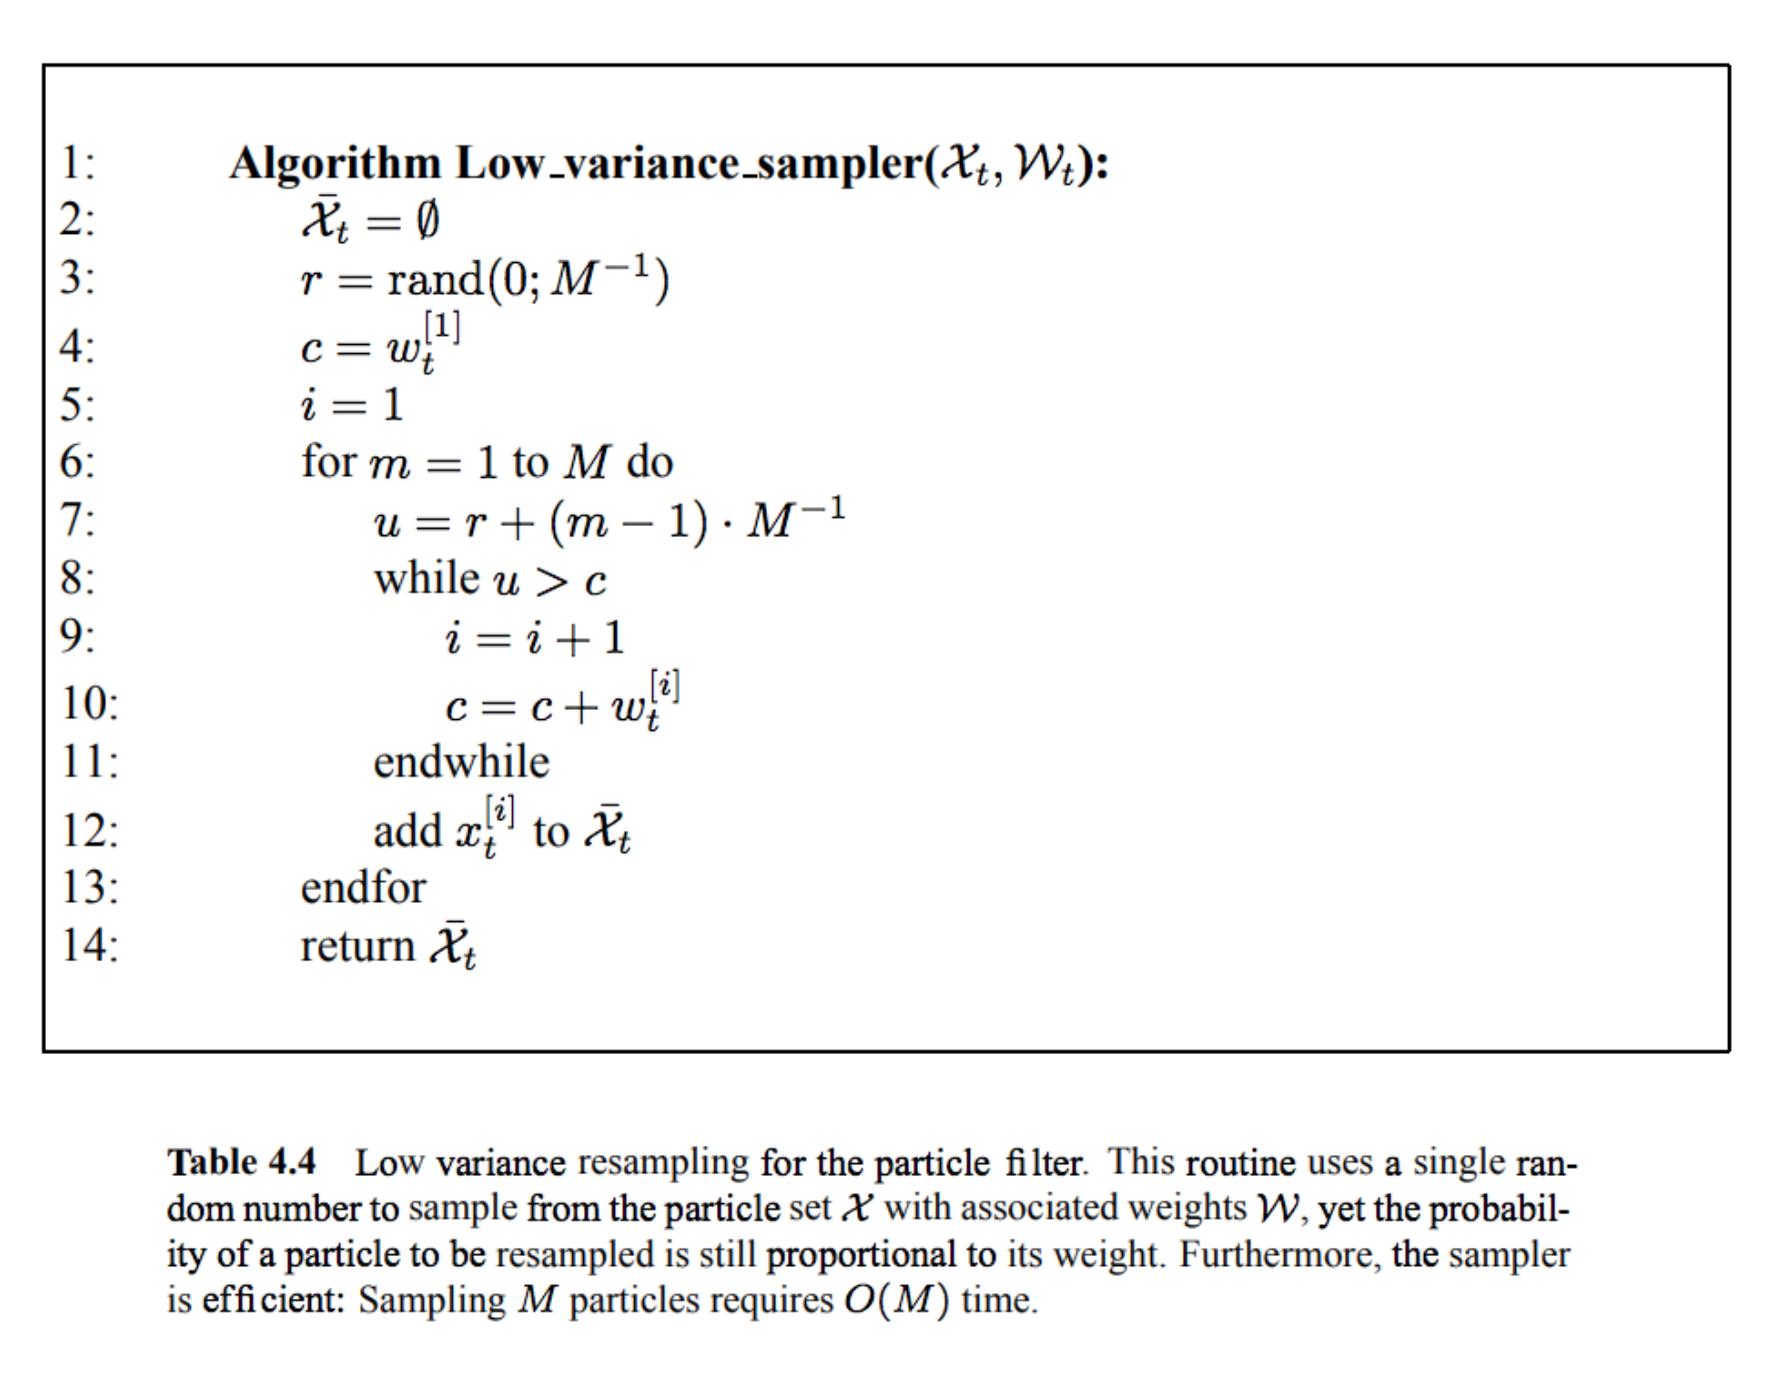
\includegraphics[width=12cm]{figs/low_var.png}
\end{figure}

% \begin{align*}
% M =& Mad \\
% A =& Awesome \\
% Fs=& Functions
% \end{align*}

%

For both methods, \textbf{make sure to vectorize computation whenever possible.}

\subsection{Re-Sampler Visualization}
We will visualize the samples that our re-sampler methods are drawing, as well as demonstrate that the low variance re-sampler does indeed have lower variance. We will repeatedly sample from a particle distribution where the weights are defined as follows:

\[
	w_i = 
	\begin{cases}
	\frac{i}{\Sigma w_i} & \text{if } i < k\\
	0 & \text{if } i >= k
	\end{cases}
\]

where $k$ is some value less than the the number of weights. The test code provided in the main method of \textbf{ReSampler.py} samples from this particle distribution \textit{trials} number of times, and then creates a histogram of how many times each particle was sampled across all trials. To run the test code, \textbf{make sure that teleop.launch is NOT launched}. Then launch \textbf{ReSampler.launch} to test that both of your re-sampling methods approximate the true sampling distribution.  The \textit{resample\_type} argument in \textbf{ReSampler.launch} can either be set to \textit{naiive} or \textit{low\_variance} according to which method you want to test. 

\subsection{Testing Particle Filter in Simulation with Teleoperation}
\label{sec:test_pf_sim_teleop}
You can test your particle filter in simulation by doing the following:

\begin{enumerate}

\item Change the \textit{map} parameter of \textit{racecar\_base\_public/racecar/launch/includes/common/map\_server.launch} to reference whichever map you want to use.
\item Launch teleop.launch: \texttt{roslaunch racecar teleop.launch}
\item Launch ParticleFilter.launch: \texttt{roslaunch lab2 ParticleFilter.launch}
\item Make sure that your ROS\_IP and ROS\_MASTER\_URI are set correctly
\item Open rviz and visualize the map, the \textit{/pf/viz/particles} PoseArray topic, and the \textit{/pf/viz/scan} LaserScan topic.
\item Click the '2D Pose Estimate' button, and click and drag on the map according to where the robot actually is in the map. All of the particles should then redistribute around this pose.
\item Teleoperate the car. The particle filter's estimate of the robot's state should approximately correspond to the true pose of the robot in the map.
\end{enumerate}


\subsection{Testing Particle Filter in Simulation with Bag File}
\label{sec:test_pf_sim_bag}
We have provided a number of bags for testing your particle filter implementation under the \textit{lab2/bags/real-floor4\_corridor} directory. These bags contain all of the data necessary to run the particle filter, as well as the output of our particle filter when processing the data. 
To test the particle filter, do the following:
\begin{enumerate}
\item Make sure that teleop.launch is not running.
\item Change the \textit{map} parameter of \textit{racecar\_base\_public/racecar/launch/includes/common/map\_server.launch} to reference the \textit{real-floor4\_corridor} map. 
\item Launch the map\_server: \texttt{roslaunch racecar map\_server.launch}
\item Launch the particle filter: \texttt{roslaunch lab2 ParticleFilter.launch}
\item Begin playing back the bag: \texttt{rosbag play <path to bag>}
\item Open rviz and visualize the map, as well as the following topics:
	\begin{itemize}
		\item The \textit{/pf/viz/inferred\_pose} Pose topic
		\item The \textit{/pf/viz/scan} LaserScan topic
		\item The \textit{/pf/ta/viz/inferred\_pose} Pose topic
	\end{itemize}
\end{enumerate} 

The output of our particle filter implementation is published to topics that are prefixed with \textit{/pf/ta/viz}, while the outputs of your implementation will publish to topics prefixed with \textit{/pf/viz}. If you view these topic in rviz, you can compare the performance of your particle filter to our implementation. Though it is unlikely that both filters will produce exactly the same results, the expected poses of both filters should be similar at all times.

\subsection{Testing Particle Filter on Robot}

We suggest that you run your particle filter code directly on the robot. To do this, you should use the scp command to copy your \textit{lab2} directory directly into the \textit{catkin\_ws/src} directory on the robot. Then run \texttt{catkin\_make} in the robot's \textit{catkin\_ws} directory.

Next, do the same procedure described in Section \ref{sec:test_pf_sim_teleop}, \textbf{except perform steps 1 through 3 on the robot instead of your computer}. Steps 4 through 7 should be done on your own computer. Note that now when you specify the initial pose in rviz, it should correspond to where the robot really is, not some arbitrary starting point in the map.

\section{Submission}

Submit all of your code and launch files.

\subsection{Motion Model}
\begin{enumerate}
\item Run the code that visualizes your motion model three times. For each run, choose a test speed, steering angle, and time interval that result in different robot motions. Submit the visualizations for all three runs.
\item Answer: How did you initially choose the noise parameter values?
\item Answer: After picking the initial values, did you tune them? If yes, how so?
\item Answer: What were your final values for these parameters?
\end{enumerate}

\subsection{Sensor Model}
\begin{enumerate}
\item Run the code that visualizes your sensor model on each of the three provided laser scan bags. Submit the visualizations for all three runs.
\item Answer: How did you initially chose the mixing weights? How did you initially choose the value of SIGMA\_HIT?
\item Answer: After picking the initial values, did you tune them? If yes, how so?
\item Answer: What were your final values for these parameters?
\end{enumerate}

\subsection{Re-Sampler}
\begin{enumerate}
\item Run the code that visualizes the re-sampler with the \textit{trials} parameter set to ten for both methods. Submit both visualizations.
\item Answer: Which of the two methods represents the true particle distribution better? How so?
\item Increase the number of trials until the sampling methods starts representing the true particle distribution equally well. Submit the visualizations for both methods.
\item Answer: At what number of trials did both methods begin to represent the true particle distribution well?
\end{enumerate}

\subsection{Particle Filter}
\begin{enumerate}
\item Record a video of your particle filter estimating the robot's state when playing back the \textit{lab2/bags/real-floor4\_corridor/full\_2x.bag} file. \textbf{Make sure to visualize all of the topics mentioned in Section \ref{sec:test_pf_sim_bag}.} Show your particle filter's estimate of the expected pose in blue, and our recorded estimate in green. Please playback and record the estimates for the \textbf{whole} bag (note that at one point the robot pauses its movement, but then continues moving shortly afterwards). Your estimates will not exactly match ours, but they should be similar at all times.

\end{enumerate}

[Robot track only] In addition, you will demo the real robot estimating its pose as it is being teleoperated. A rubric containing detailed requirements will be released shortly.

\end{document}
